\documentclass{snapshotmfo}

\categorizationmath{algebra and number theory,analysis,discrete mathematics and foundations,geometry and topology,numerics and scientific computing,probability theory and statistics} %at least one must be chosen. 
\categorizationconnect{chemistry and earth science,engineering and technology,finance,humanities and social sciences,life science,physics,reflections on mathematics} %can be void.
\license{CC-BY-SA-4.0} %recommended
\snapshotid{139}{1950}
\junioreditor{Some One}{junior-editors@mfo.de}
\senioreditor[f]{Carla Cederbaum}{senior-editor@mfo.de}
\director[m]{Gerhard Huisken}
\usepackage[utf8]{inputenc}
\usepackage{amsmath,amssymb}
%%% Wrap text around tables and figures:
\usepackage{wrapfig}

%\usepackage[ngerman]{babel}
\usepackage[USenglish]{babel}

\author{Test Author}
\title{wrapfig}
\begin{document}

\begin{abstract}
Does the latex package wrapfig work?
\end{abstract}

\begin{wrapfigure}{I}{0.6\textwidth}
\centering
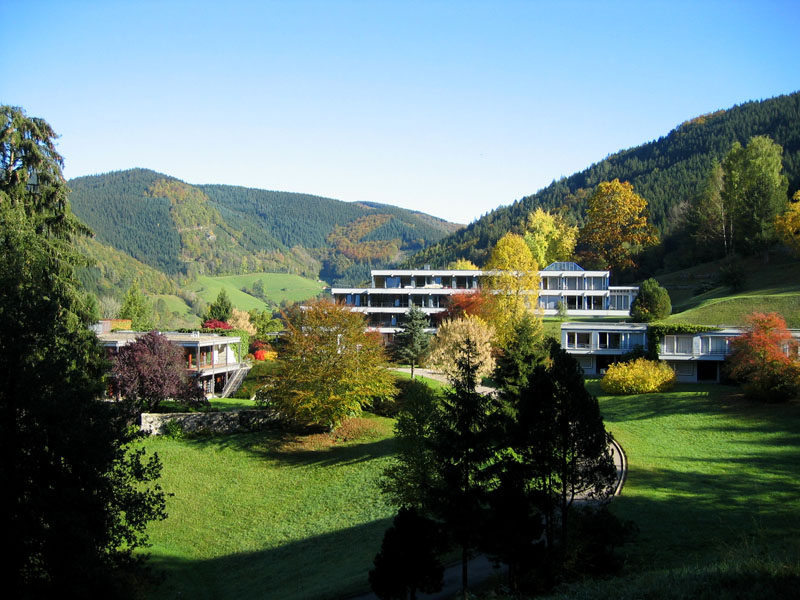
\includegraphics[width= 0.6 \textwidth]{mfo.jpg}
\caption{An image scaled to 60\% of the textwidth.}
\end{wrapfigure}

As the packages wrapfig and lipsum do not harmonize any more,
the following dummy text is inserted directly:

Lorem ipsum dolor sit amet, consectetur adipiscing elit. Duis in massa non
augue imperdiet fringilla. In mauris sapien, imperdiet non bibendum sed,
mollis a elit. Proin aliquet nisi vel felis viverra, eget rutrum sem venenatis.
Vivamus porta purus sed magna faucibus tempus. Mauris dictum eros mi, eu
malesuada ex feugiat vitae. Pellentesque ornare, lectus non mattis semper,
orci libero varius risus, sed mollis massa augue id libero. Donec aliquet ut
purus ut mattis. Maecenas a eleifend neque, lacinia tristique ante. Sed
dignissim massa ut metus placerat, et bibendum urna vestibulum. Nam in suscipit
lorem. Morbi in erat dolor. Nam ac consectetur eros.

\end{document}
